\chapter{Cell Monitoring}

\hspace{0.5cm} 
Using new, cycle-aged, calendar-aged, or over-discharged cells, the shortcomings of cell voltage, surface temperature, and electrolyte resistance monitors to detect and predict cell mismatch is verified experimentally. These results highlight that bad and normal cells are nearly identical in their $E_{cv}$ and $T_{surf}$ values, while high-frequency impedance is concurrently influenced by electrolyte temperature, cell aging and changes in Li+ concentration. 

\section{Cell Voltage Monitor}

\hspace{0.5cm}
$E_{cv}$ monitoring is a commonly incorporated feature in conventional BMS. Its main role in a BMS is to ensure that no cell in the battery exceeds preset upper and lower limits, respectively. During current flow (when charging or discharging), $E_{cv}$ is dominated by three different polarization effects: 1) activation and diffusion at the anode and the cathode, 2) resistive drop across the electrolyte, with relatively insignificant contributions from 3) foreign-object-debris ($FOD$). FOD refers to any nonfunctional material that despite careful cell manufacturing may find its way into the cell. For example, FOD include copper and aluminum particulates from current collectors. FOD can cause internal short circuit, chemical changes induced by over-discharge, and chemical and physical changes after cycle and calendar aging. As a result, $E_{cv}$ of cells with FOD, over-discharge and age abnormalities will be quite similar to those of cells without those abnormalities. FOD, over-discharge, and aging are the main reasons why cells become mismatched; however, cell voltage monitoring alone cannot identify cell mismatch.

\vspace{0.5cm}
The data in Figure \ref{emf1} demonstrate that in a six-cell battery with five aged cells and one over-discharged cell, the $E_{cv}$ of all six cells remained close (standard deviation under $\pm$5 mV), down to 30\% SoC during discharge, and at all SoC during charge. Only below 20\% SoC did the cell voltages start to deviate markedly from each other, with the over-discharged (bad) cell deviating most at full discharge. At full discharge, the bad cell was at 2.387 V, i.e., 313 mV below the manufacturer-recommended 2.7 V limit for the cell, while the voltage of the entire battery reached only its lower limit (16.2V), falsely suggesting that each cell was at the 2.7 V limit ($2.7V\ast6=16.2V$). A cell-voltage monitor in a BMS is thus not always capable of identifying mismatched and over-discharged cells, and will miss bad cells discharging far below their recommended limit, which might cause a battery fire.

\begin{figure}
	\includegraphics[width=11cm,height=8cm]{figures/emf_monitor.png}
	\centering
	\caption{
		Cell voltages(discharge and charge of a six cell Li-ion battery containing five matched and one over-discharged cell.)}\label{emf1}
\end{figure}

\section{Surface Temperature Monitor}

\hspace{0.5cm}
Next monitor method is cell surface temperature $T_{surf}$ in order to identify cell mismatching. Battery voltage (indicating the discharge{/}charge cycle) and surface temperature variations for one normal and the bad (previously over-discharged) cell in the six cell battery from Figure \ref{emf1} are plotted in Figure \ref{tem1} The surface temperatures of the normal and over discharged cells were virtually identical until the battery was fully drained (at 687 min time point). For a completely drained battery, the surface temperature of the bad cell deviates by no more than one degree from normal cell temperature ($24^oC$). In other words, surface-mounted temperature sensors can barely discriminate an over-discharged (i.e., mismatched) cell from normal cells. Similarly, for batteries with new and cycle-aged cells, individual cell $T_{surf}$ values were identical to each other. In addition to not being adequate in discriminating bad cells from normal ones, surface-mounted sensors have several more shortcomings. $T_{surf}$ sensors are slow in responding to changes in the discharge currents flowing through the cell and they cannot identify when the cell is being overcharged. Furthermore, when a battery is rapidly charged or discharged, $T_{surf}$ values do not indicate impeding damage to the interior of the cell. For example, through the discharge–charge cycle at $1^oC$ rate of a three-cell battery, $T_{surf}$ remained well within $20^oC$ to $40^oC$ (see Figure \ref{tem2}). This temperature range is considered “safe” by most battery safety standards. However, the cell’s internal temperature exceeded $60^oC$, less than $20^o$ below $80^oC$, considered unsafe by most standards.

\begin{figure}[H]
	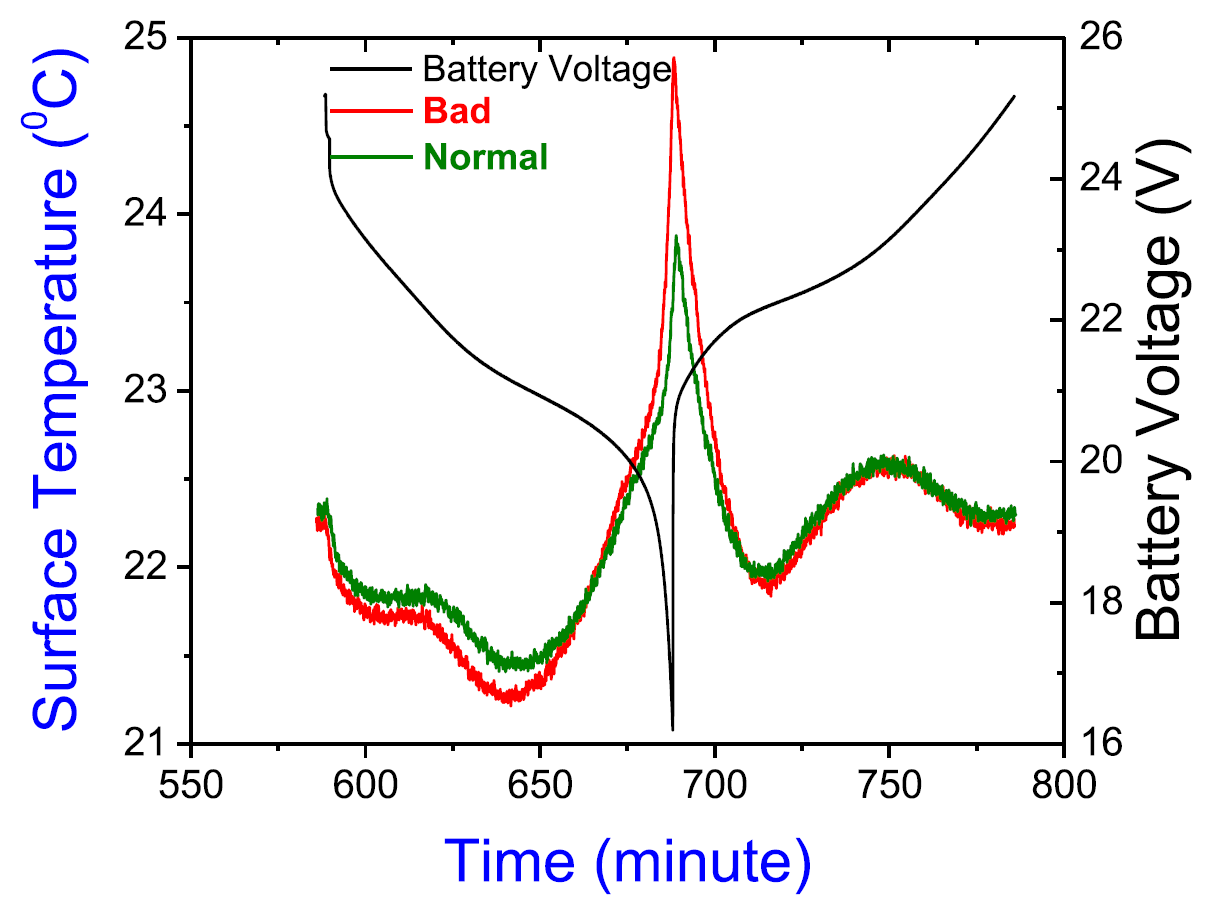
\includegraphics[width=11cm,height=8cm]{figures/tem1}
	\centering
	\caption{Surface temperatures of one aged (normal, green) and one over-discharged (bad, red) cell.}\label{tem1}\vspace{0.5cm}

	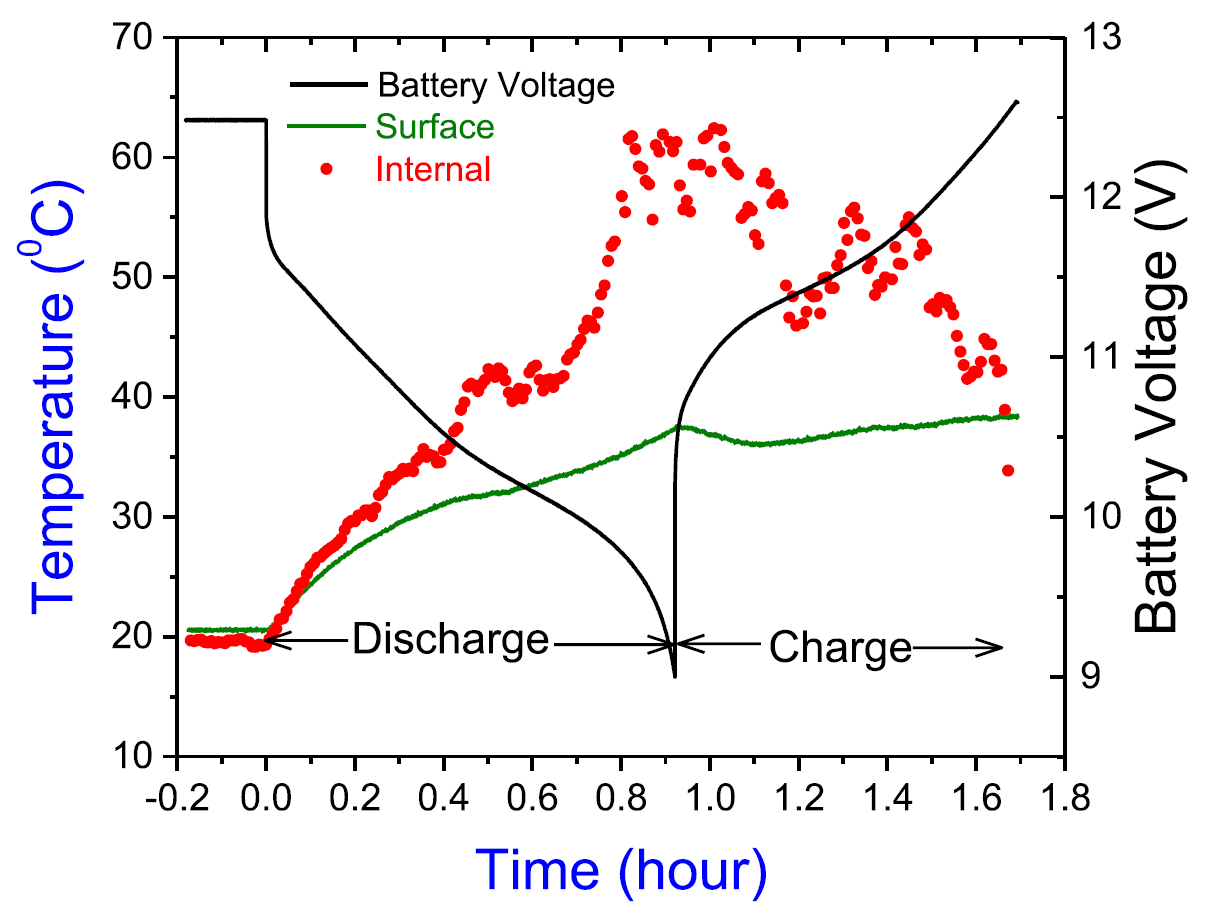
\includegraphics[width=11cm,height=8cm]{figures/tem2}
	\centering
	\caption{
		Surface temperature (green) and internal (anode) temperature (red) of one of the cells in a cycle-aged three-cell battery.}\label{tem2}
\end{figure}

\section{Electrolyte Resistance Monitor}

\begin{figure}[H]
	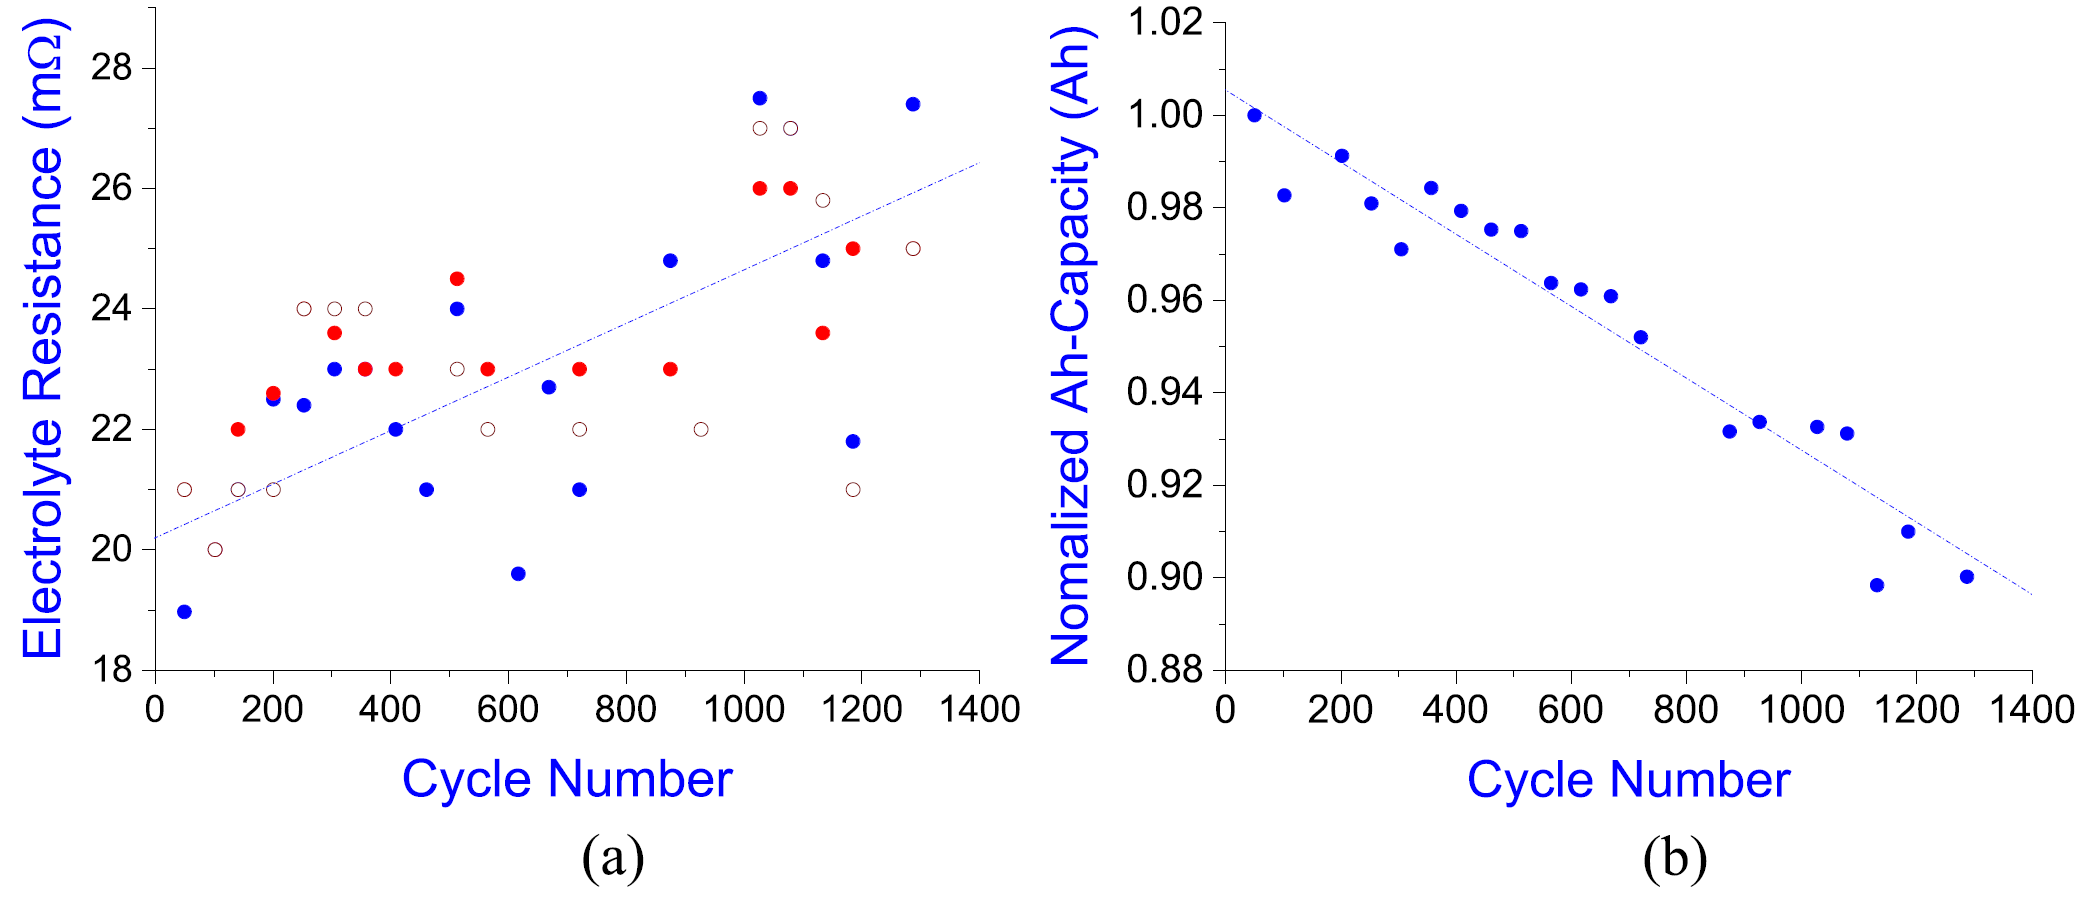
\includegraphics[width=16cm,height=7cm]{figures/electrolyte1}
	\centering
	\caption{(a) Effect of cycle life on electrolyte resistance, $R_s$ , in three identical Li-ion cells. (b) Ah-capacity as a function of cycle life for one of the three cells.} \label{electrolyte1}
\end{figure}

\hspace{0.5cm}
$R_s$  reportedly serves two purposes: 1) to identify a cell’s internal temperature; 2) to estimate cell aging and health. In both cases, $R_s$ is determined from measured cell impedance at a single frequency. While single-frequency impedance monitoring can estimate cell cycle-life aging, it is valid only if impedance is measured after the cell is rested for extended time at constant ambient temperature (see Figure \ref{electrolyte1}). Furthermore, $R_s$ can be correlated to the temperature of the electrolyte only if age-induced changes in electrolyte resistance are ignored and no current is flowing through the cell. For example, Li+ cations, released into the electrolyte from the anode during discharge, are taken into the cathode; the opposite process occurs during charge. However, the rates of release and intake, reflecting the anode and cathode reaction kinetics, respectively, differ (the release rate is higher than the intake). The rate differences between the two electrodes result in $[Li+]$ buildup in the electrolyte. $[Li+]$ change during discharge and charge results in a change in electrolyte resistance.

\vspace{0.5cm}
In the example shown [see Figure \ref{electrolyte2} (a)], during cell charge and discharge at $C/2$-rate, $R_s$ varied between 22.7 and 25 $m\Omega$. This 14\% variation between $R_s$ maximum and minimum is comparable to the 30\% change observed due to cycle life aging [see Figure \ref{electrolyte1} (a)]. Therefore, monitoring cell aging from high-frequency impedance data may be feasible only if impedance is measured when the cell is at rest, and care is taken to maintain the cell at the same internal temperature between each measurement [see Figure \ref{electrolyte1} (a)]. The variation in $R_s$ can be caused by changes in electrolyte temperature as well as changes in $[Li+]$ in the electrolyte. If impedance measurements are used in estimating electrolyte temperature during charge and discharge, the current-induced changes in $[Li+]$ will introduce errors in those estimates, as demonstrated in the discrepancy between the cell internal temperature (estimated from high-frequency impedance) and the surface temperature [see Figure \ref{electrolyte2} (b)]. Compared to $T_{surf}$ , the internal temperature behaved differently after an initial rise to $28^oC$ during discharge, it subsequently dropped. The drop in internal temperature is an artifact, best explained by the differences in reaction kinetics between the anode and the cathode and $[Li+]$ changes during discharge.

\begin{figure}[H]
	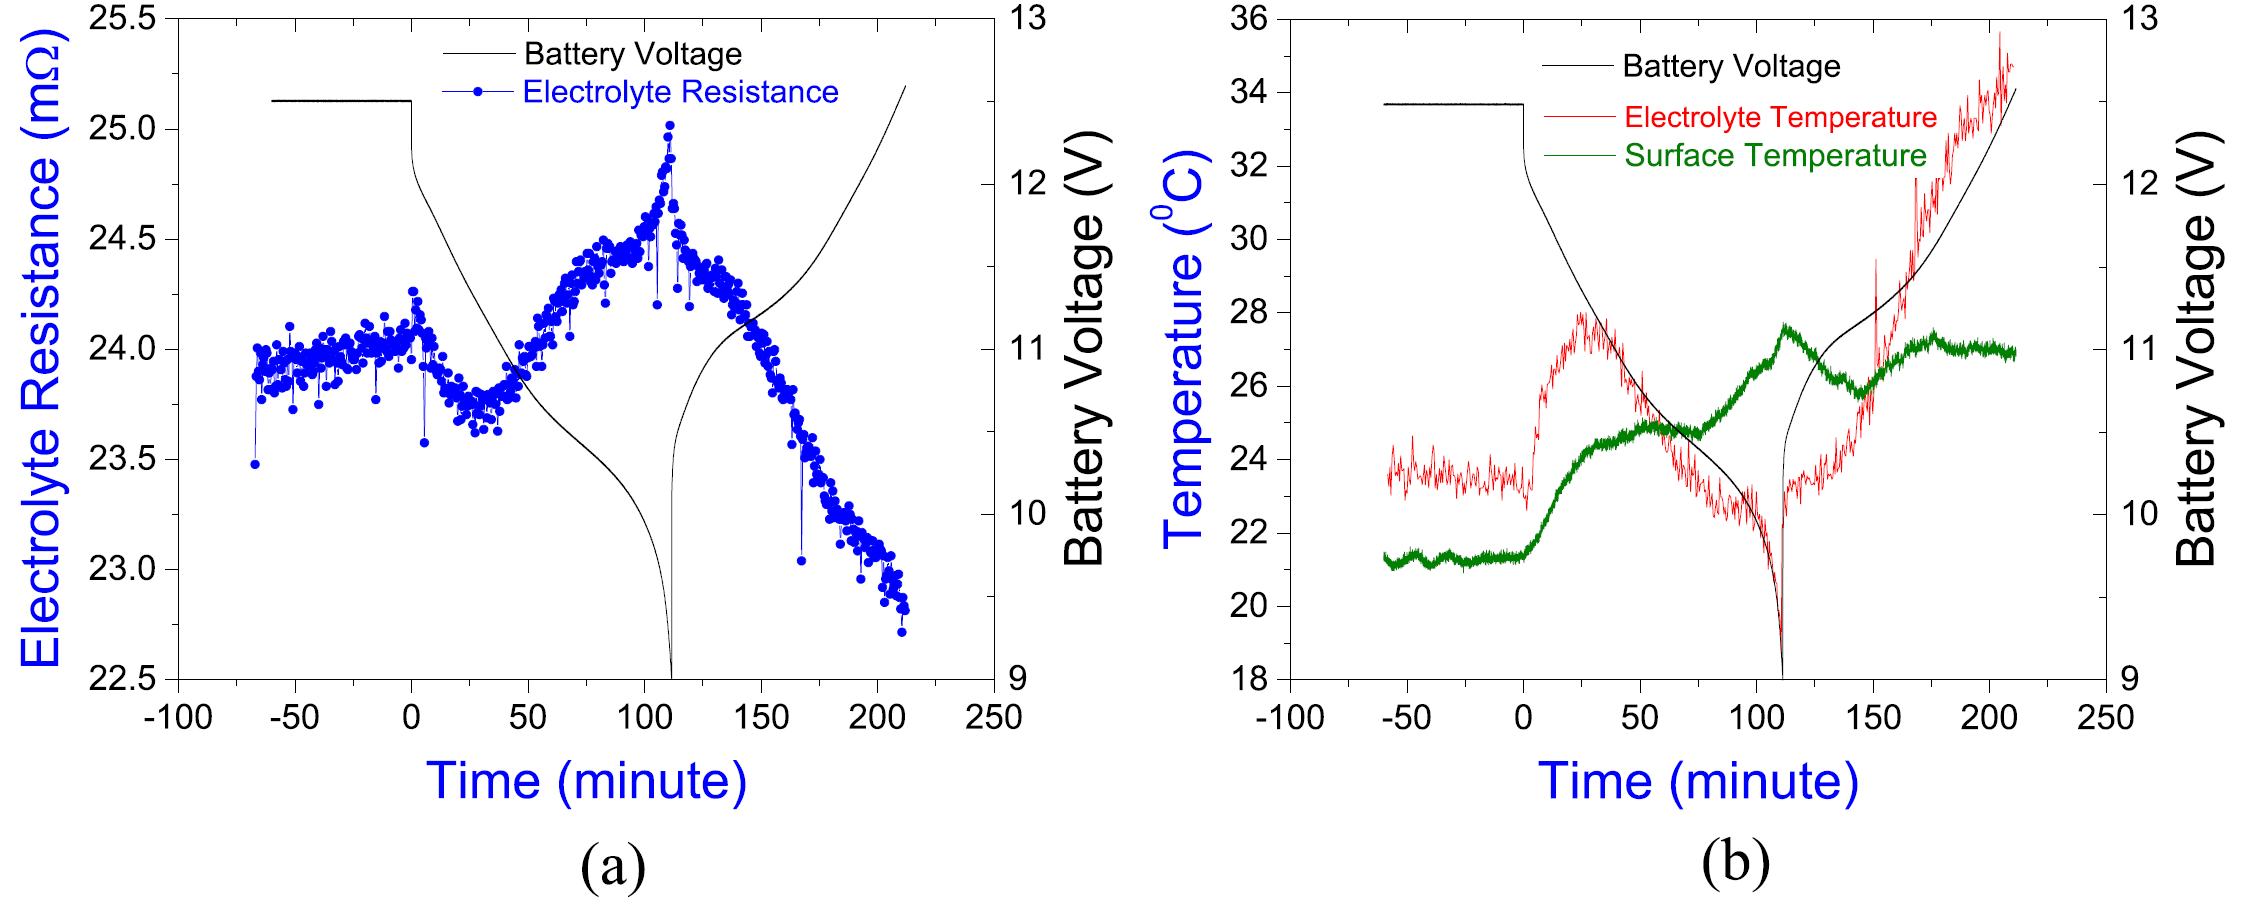
\includegraphics[width=16cm,height=6cm]{figures/electrolyte2}
	\centering
	\caption{
		(a) Electrolyte resistance, Rs of one cell during a single cycle of discharge{/}charge of a new and matched three-cell battery (b) Internal temperature (red) of the same cell and surface temperature (green).} \label{electrolyte2}
\end{figure}

\section{Impedence approach to identify Cell miss-match}

\begin{figure}[H]
	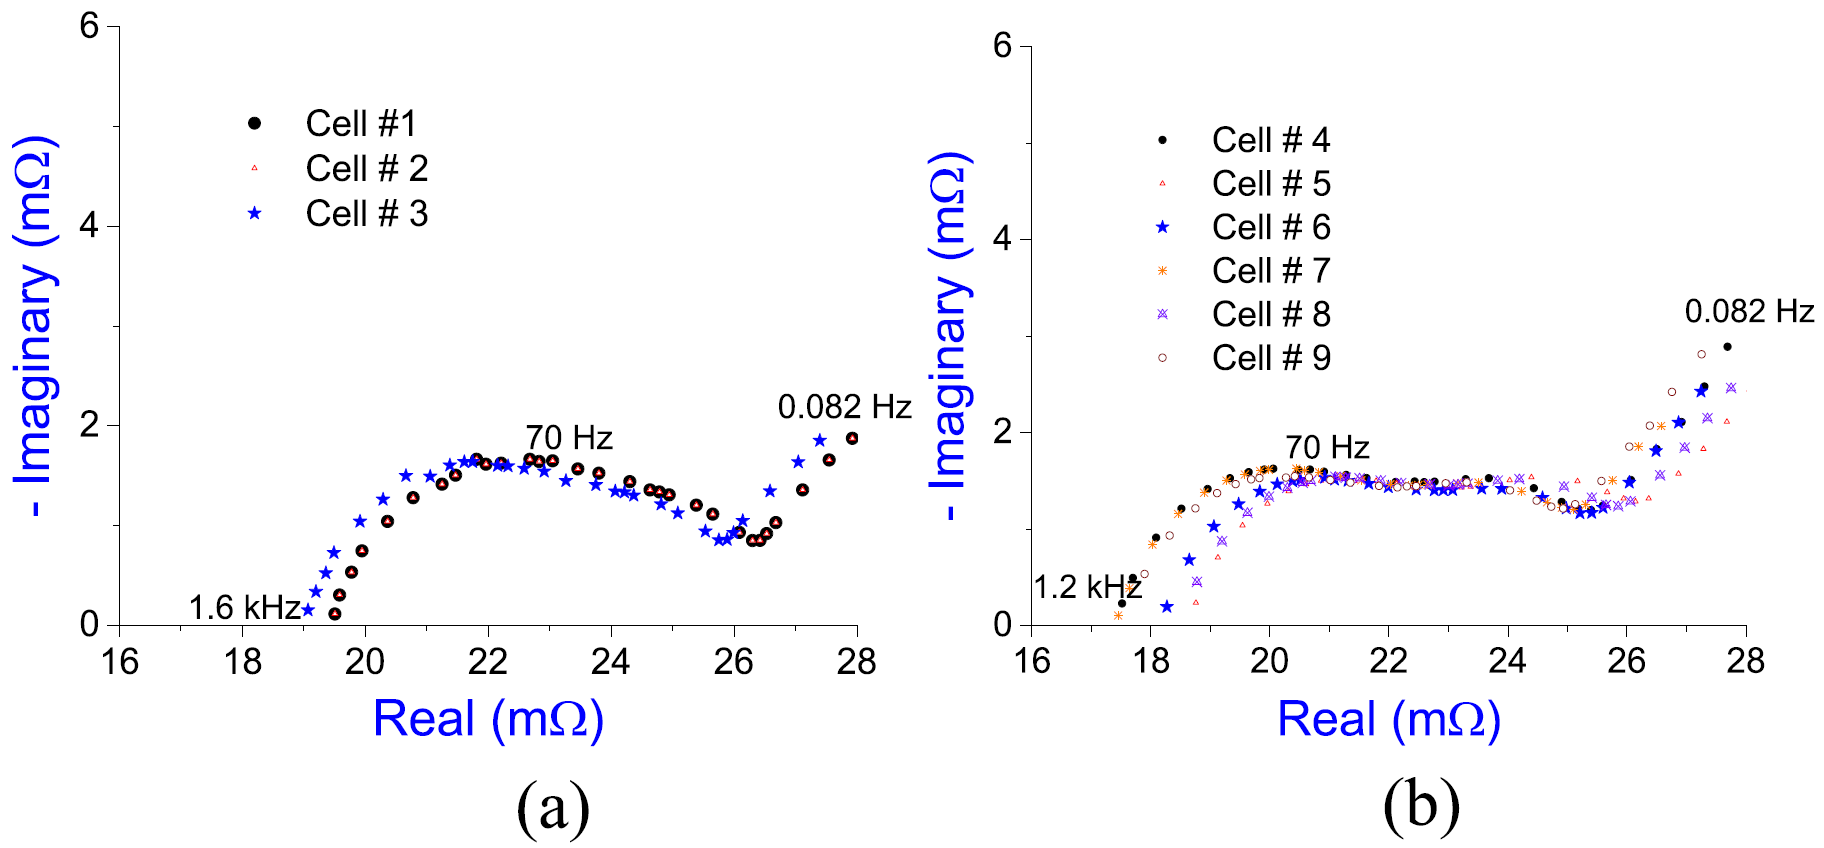
\includegraphics[width=16cm,height=7cm]{figures/impedence1}
	\centering
	\caption{Impedance behavior of cells in different Li-ion batteries containing: (a) three new, matched cells; (b) six matched, calendar-aged cells.} \label{impedence1}
\end{figure}

\hspace{0.5cm}
A Li-ion cell is a multi-component system, consisting of an anode, cathode, electrolyte, separator, and current collectors. The solid-electrolyte-interphase (SEI) layer is most sensitive to temperature and least sensitive to SoC. Current flow changes SEI layer’s temperature, therefore measuring the impedance allows to monitor the cell’s anode and cathode temperatures. Low-frequency impedance is influenced by both SoC and internal temperature. However, separating their effects can be challenging. $R_s$ , best identified as high-frequency impedance, is also sensitive to temperature, $[Li+]$ and cell aging. Thus, a multi-frequency impedance meter equipped to measure both phase shift and amplitude is required to discern changes occurring in the anode, cathode, and the electrolyte.

\begin{figure}[H]	
	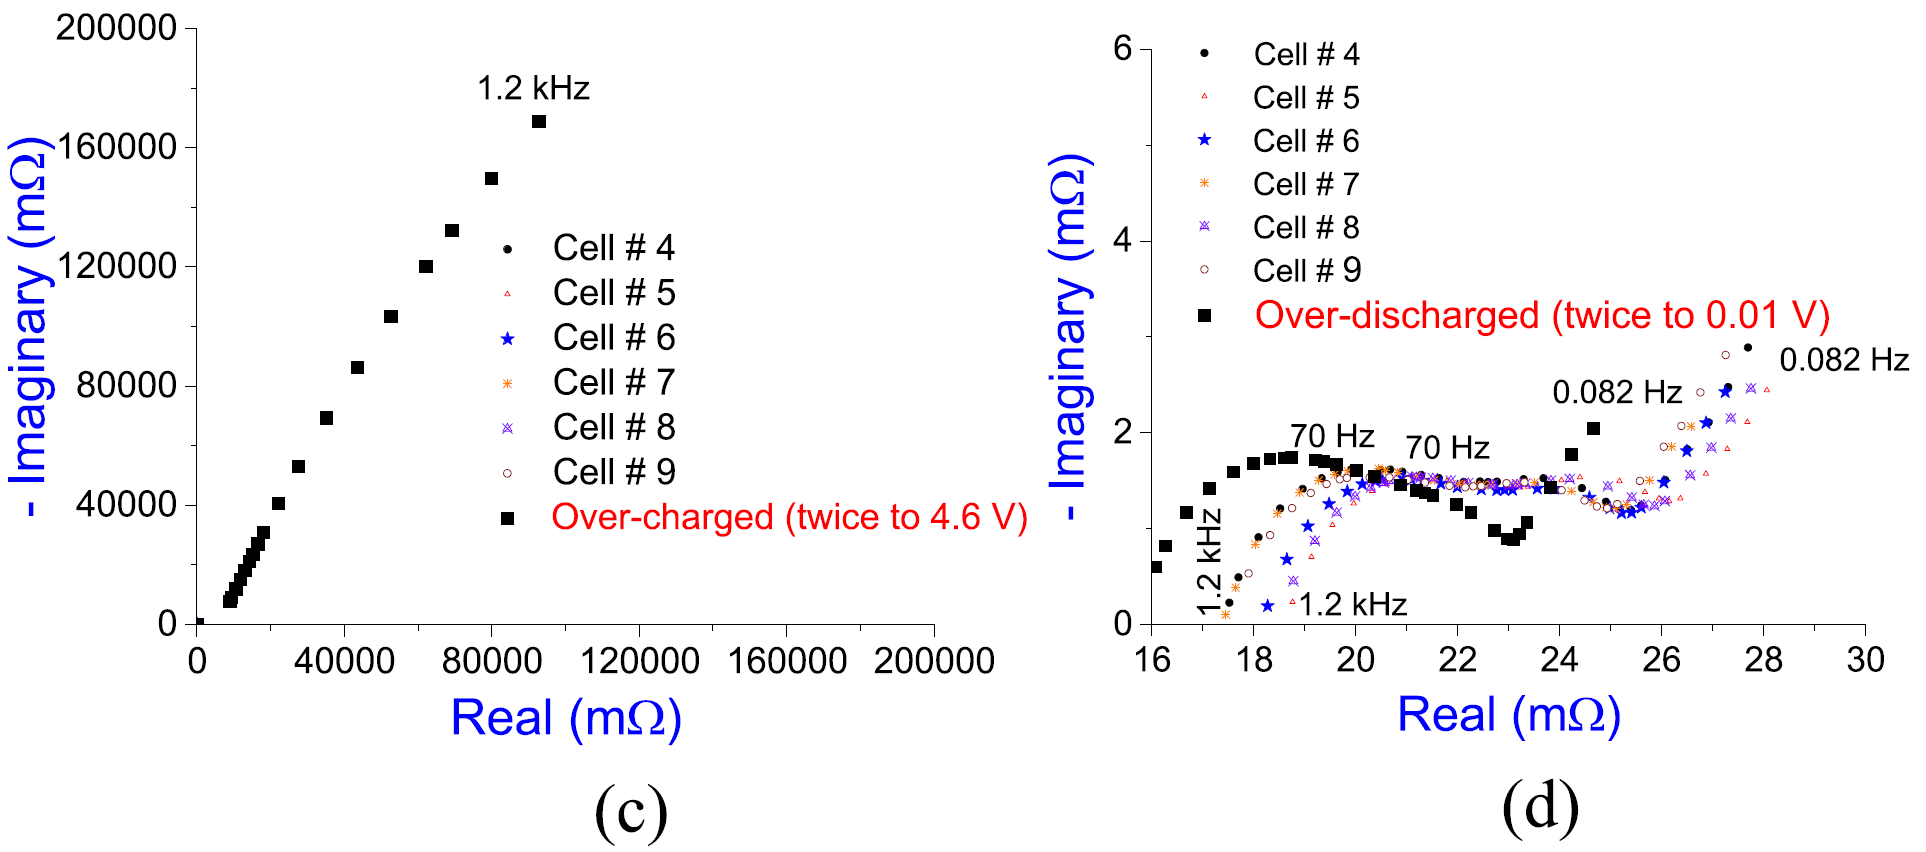
\includegraphics[width=16cm,height=7cm]{figures/impedence2}
	\centering
	\caption{Impedance behavior of cells in different Li-ion batteries containing: (a) five matched, calendar-aged cells and one overdischarged cell; (b) five matched, calendar-aged cells and one overcharged cell.} \label{impedence2}
\end{figure}

Figure \ref{impedence1} (a) shows impedance data for three cells in a three-cell battery matched within $\pm$0.5\%. Figure \ref{impedence1} (b) shows impedance data for each of the six cells in a six-cell battery after aging. Individual cell’s impedance drifted from its original value by more than 6\% [see Figure \ref{impedence1} (b)], while the spread in impedance values after aging also increased. Also examined are two modified six-cell batteries that had five cells aged as the ones in Figure \ref{impedence1} (b), with the sixth cell replaced by an over-discharged cell, or by an overcharged cell, respectively. The purpose of deliberately over-discharging one cell in the six-cell battery is to demonstrate: 1) cell voltage monitors are unable to identify an over-discharged cell in the battery; and 2) impedance technique can identify the over-discharged cell event, before the event causes internal short. The impedance of the over-discharged cell after resting the cell overnight at 50\% SoC compared to the impedance of the five normal aged cells is markedly different [see Figure \ref{impedence2} (a)].  Figure \ref{impedence2} (b) shows impedance data for all six cells in the battery with one cell overcharged twice by charging up to 4.6 V (4.2 V is the upper limit for normal charge). The impedance of the over-discharged cell is 100000 times larger than the rest of the cells.






